\documentclass{article}

\usepackage[polish]{babel}
\usepackage[T1]{fontenc}
\usepackage{tabularx}
\usepackage{amsfonts}
\usepackage{amsmath}
\usepackage{mathtools}
\usepackage{enumitem}
\usepackage{graphicx}
\usepackage{algpseudocode}

\begin{document}
    \begin{titlepage}
        \title{Algorymy metaheurystyczne}
        \author{Mateusz Chęciński, Mateusz Tofil}
        \maketitle
    \end{titlepage}

    \section{Wprowadzenie}

    Celem tej listy było zapoznanie się z algorytmem przeszukiwania z
    zabronieniami (z ang. Tabu search). 

    \noindent Język programowania: Python 3.10

    \section{Porównanie otoczeń: insert, invert, swap}

    W celu zbadania jakie otoczenie jest najlepsze z
    powyższych 3, przeprowadziliśmy eksperymenty wywołując
    metode ze zmienionym parametrem początkowym. Wszystkie
    eksperymetry były przeprowadzone dla tej samej instacji
    wraz z tym samym rozwiązaniem początkowym.

    \begin{figure}[h!]
        \centering
        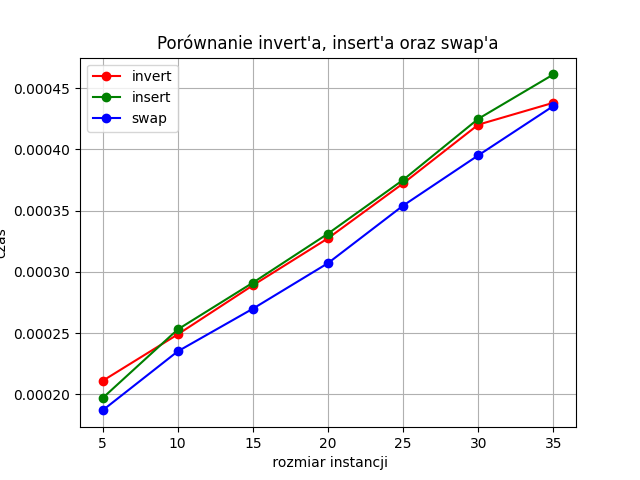
\includegraphics[width=11cm]{./spr2img/Figure_1.png}
        \caption{Porównanie otoczeń}
    \end{figure}

    Jak możemy zauważyć, dla wszystkich przeprowadzonych
    przez nas intacji, otocznie \emph{swap} okazało się być
    najelpszym. Pozostałe otoczenia, też nie są źle. Wszystkie
    otoczenia działają w czasie $\mathcal{O}(n)$ i różnią się tylko
    stałą, najmniejszą stałą posiada \emph{swap}

    \section{Czy długość listy Tabu ma znaczenie? }

    Chclieśmy upewnić się, czy zwiększając długość listy
    Tab'u otrzymamy lepszy wynik. tj cykl o najmniejszym koszcie
    w chwili kończenia algortmy. Doskonale wiemy, że jakbyśmy
    zwiększyli sam rozmiar listy tabu to algorytm wykonywał by
    się znacznie dłużej. Dlatego zdecydowaliśmy się, że podzielimy
    wartość (koszt) cyklu na zakończeniu algorytmy przez czas w jakim
    otrzymaliśmy wynik.

    \begin{figure}[h!]
        \centering
        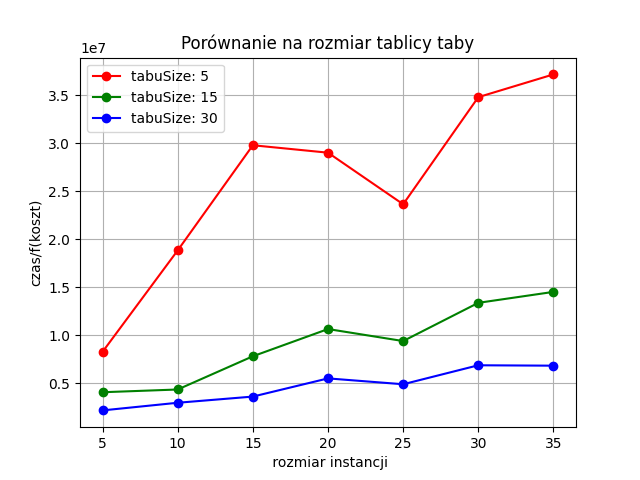
\includegraphics[width=11cm]{./spr2img/Figure_4.png}
        \caption{Porównanie otoczeń}
    \end{figure}

    Wyszło, tak jak zakładaliśmy, czyli mimo, że algorytm dłużej
    pracował, (im wieksza liczba tabu, tym dłużej działą), daje lepsze
    wyniki. Zatem warto jest poczekać odpowiednio dłużej aby otrzymać
    lepszy wynik.

\end{document}